\documentclass[14pt]{beamer}
\usepackage{omi-template}
\usepackage{hyperref}

\usepackage{calc}
\newlength{\myscalewidth}
\newcommand{\scaletowidth}[2]{%
\setlength{\myscalewidth}{\widthof{#2}}%
\pgfmathsetmacro{\myscaleratio}{#1/\myscalewidth}%
\scalebox{\myscaleratio}{#2}}

\makeatletter
\define@key{beamerframe}{nofills}[true]{% top
  \beamer@frametopskip=0pt\relax%
  \beamer@framebottomskip=0pt\relax%
  \beamer@frametopskipautobreak=\beamer@frametopskip\relax%
  \beamer@framebottomskipautobreak=\beamer@framebottomskip\relax%
  \def\beamer@initfirstlineunskip{%
    \def\beamer@firstlineitemizeunskip{%
      \vskip-\partopsep\vskip-\topsep\vskip-\parskip%
      \global\let\beamer@firstlineitemizeunskip=\relax}%
    \everypar{\global\let\beamer@firstlineitemizeunskip=\relax}}
}
\makeatother


\usepackage{tikz}
\usetikzlibrary{calc}
\usetikzlibrary{shadings}
\usetikzlibrary{arrows, decorations.markings}
\usetikzlibrary{shapes.arrows}
\usetikzlibrary{positioning,fadings,through}

\newcounter{a}
\newcounter{b}

\newcommand{\slice}[5]{
  \pgfmathparse{0.5*#1+0.5*#2}
  \let\midangle\pgfmathresult

  % slice
  \draw[thick,fill=#5] (0,0) -- (#1:1) arc (#1:#2:1) -- cycle;

  % outer label
  %\node[label=\midangle:#4] at (\midangle:0.5) {};

  % inner label
  \pgfmathparse{min((#2-#1-10)/110*(-0.3),0)}
  \let\temp\pgfmathresult
  \pgfmathparse{max(\temp,-0.5) + 0.8}
  \let\innerpos\pgfmathresult
  \node at (\midangle:\innerpos) {\parbox{1in}{\begin{center}#3 \\ \scriptsize #4\end{center}}};
}

\tikzfading[name=fade right,
  left color=transparent!0, right color=transparent!100]
\tikzfading[name=fade left,
  right color=transparent!0, left color=transparent!100]
\tikzfading[name=fade down,
  bottom color=transparent!0, top color=transparent!100]
\tikzfading[name=fade up,
  top color=transparent!0, bottom color=transparent!100]
\tikzfading[name=fade out,
  inner color=transparent!0, outer color=transparent!100]


\def\shadowradius{0.025\textwidth}
\def\zerodistance{1pt}
%
\newcommand\drawshadowbis[1]{
  \begin{pgfonlayer}{shadow}
    \fill[fill=white] ($(#1.south west)+(-\zerodistance,-\zerodistance)$) rectangle ($(#1.north east)+(\zerodistance,\zerodistance)$);

    \begin{scope}
      \clip ($(#1.south west)$) rectangle ++(-\shadowradius,-\shadowradius);
      \fill[fill=white,path fading=fade out]
        ($(#1.south west)$) circle (\shadowradius);
    \end{scope}

    \begin{scope}
      \clip ($(#1.south east)$) rectangle ++(\shadowradius,-\shadowradius);
      \fill[fill=white,path fading=fade out]
        ($(#1.south east)$) circle (\shadowradius);
    \end{scope}

    \begin{scope}
      \clip ($(#1.north west)$) rectangle ++(-\shadowradius,\shadowradius);
      \fill[fill=white,path fading=fade out]
        ($(#1.north west)$) circle (\shadowradius);
    \end{scope}

    \begin{scope}
      \clip ($(#1.north east)$) rectangle ++(\shadowradius,\shadowradius);
      \fill[fill=white,path fading=fade out]
        ($(#1.north east)$) circle (\shadowradius);
    \end{scope}

    \fill[path fading=fade up,fill=white] ($(#1.south west)+((0,-\shadowradius)$) rectangle ($(#1.south east)$);
    \fill[path fading=fade right,fill=white] ($(#1.south east)$) rectangle ($(#1.north east)+((\shadowradius,0)$);
    \fill[path fading=fade down,fill=white] ($(#1.north west)$) rectangle ($(#1.north east)+((0,\shadowradius)$);
    \fill[path fading=fade left,fill=white] ($(#1.south west)$) rectangle ($(#1.north west)+(-\shadowradius,0)$);
  \end{pgfonlayer}
}

\pgfdeclarelayer{shadow}
\pgfsetlayers{shadow,main}

\begin{document}

%%%%%%%%%%%%%%%%%%%%%%%%%%%%%%%%%%%%%%%%%%%%%%%%%%%%%%%%%%%%%%%%
\begin{frame}[nofills]

  \vfill

  \scaletowidth{\textwidth}{\textbf{Ohio Math Initiative}}

  \begin{center}
    \textit{Subgroup 3 Update} \\
    January 20, 2017
  \end{center}

  \color{dark}

  \vfill
  \hrule
  \vspace{-12pt}

  \begin{center}
    Communication, Outreach and Engagement Co-leads
  \end{center}

  \vspace{-12pt}

  \footnotesize 
  \begin{columns}
    \begin{column}{0.4\textwidth}
      Jim Fowler \\
      The Ohio State University \\
      \texttt{fowler.291@osu.edu}
    \end{column}
    \begin{column}{0.4\textwidth}
      Michelle Younker  \\
      Owens Community College \\
      \texttt{michelle\_younker@owens.edu} \\
    \end{column}
  \end{columns}

\end{frame}

%%%%%%%%%%%%%%%%%%%%%%%%%%%%%%%%%%%%%%%%%%%%%%%%%%%%%%%%%%%%%%%%
\begin{frame}
  \frametitle{Subgroup 3}

  Subgroup 3 continues to
  \begin{itemize}
  \item communicate the work of the OMI,
  \item engage mathematicians and others in discussions about rethinking post-secondary mathematics, \textcolor{gray}{and}
  \item engage others in discussions about the work of OMI
  \end{itemize}

\end{frame}



%%%%%%%%%%%%%%%%%%%%%%%%%%%%%%%%%%%%%%%%%%%%%%%%%%%%%%%%%%%%%%%%
\begin{frame}
\frametitle{Accomplishments since January 2016}

\textbf{Developing ideas for Fast Facts publications}

Possible future topics include
\begin{itemize}
\item Open education resources (OER),
\item work with K-12 sector,
\item Quantitative Reasoning implementation, \textcolor{gray}{and}
\item updates of OTM learning outcomes.
\end{itemize}

\end{frame}


%%%%%%%%%%%%%%%%%%%%%%%%%%%%%%%%%%%%%%%%%%%%%%%%%%%%%%%%%%%%%%%%
\begin{frame}
\frametitle{Accomplishments since January 2016}

\textbf{Continuing to share Ohio's work across the state and nation}

Presentations include the
\begin{itemize}
\item Bridges to Success workshops, 
\item TPSE-Math meetings, 
\item OHAAA meeting,
\item MAA-Ohio Section,
\item OhioMATYC, \textcolor{gray}{and}
\item AMATYC.
\end{itemize}

\end{frame}

%%%%%%%%%%%%%%%%%%%%%%%%%%%%%%%%%%%%%%%%%%%%%%%%%%%%%%%%%%%%%%%%
\begin{frame}
\frametitle{Accomplishments since January 2016}

\textbf{Continuing to share Ohio's work via video}

\begin{center}
  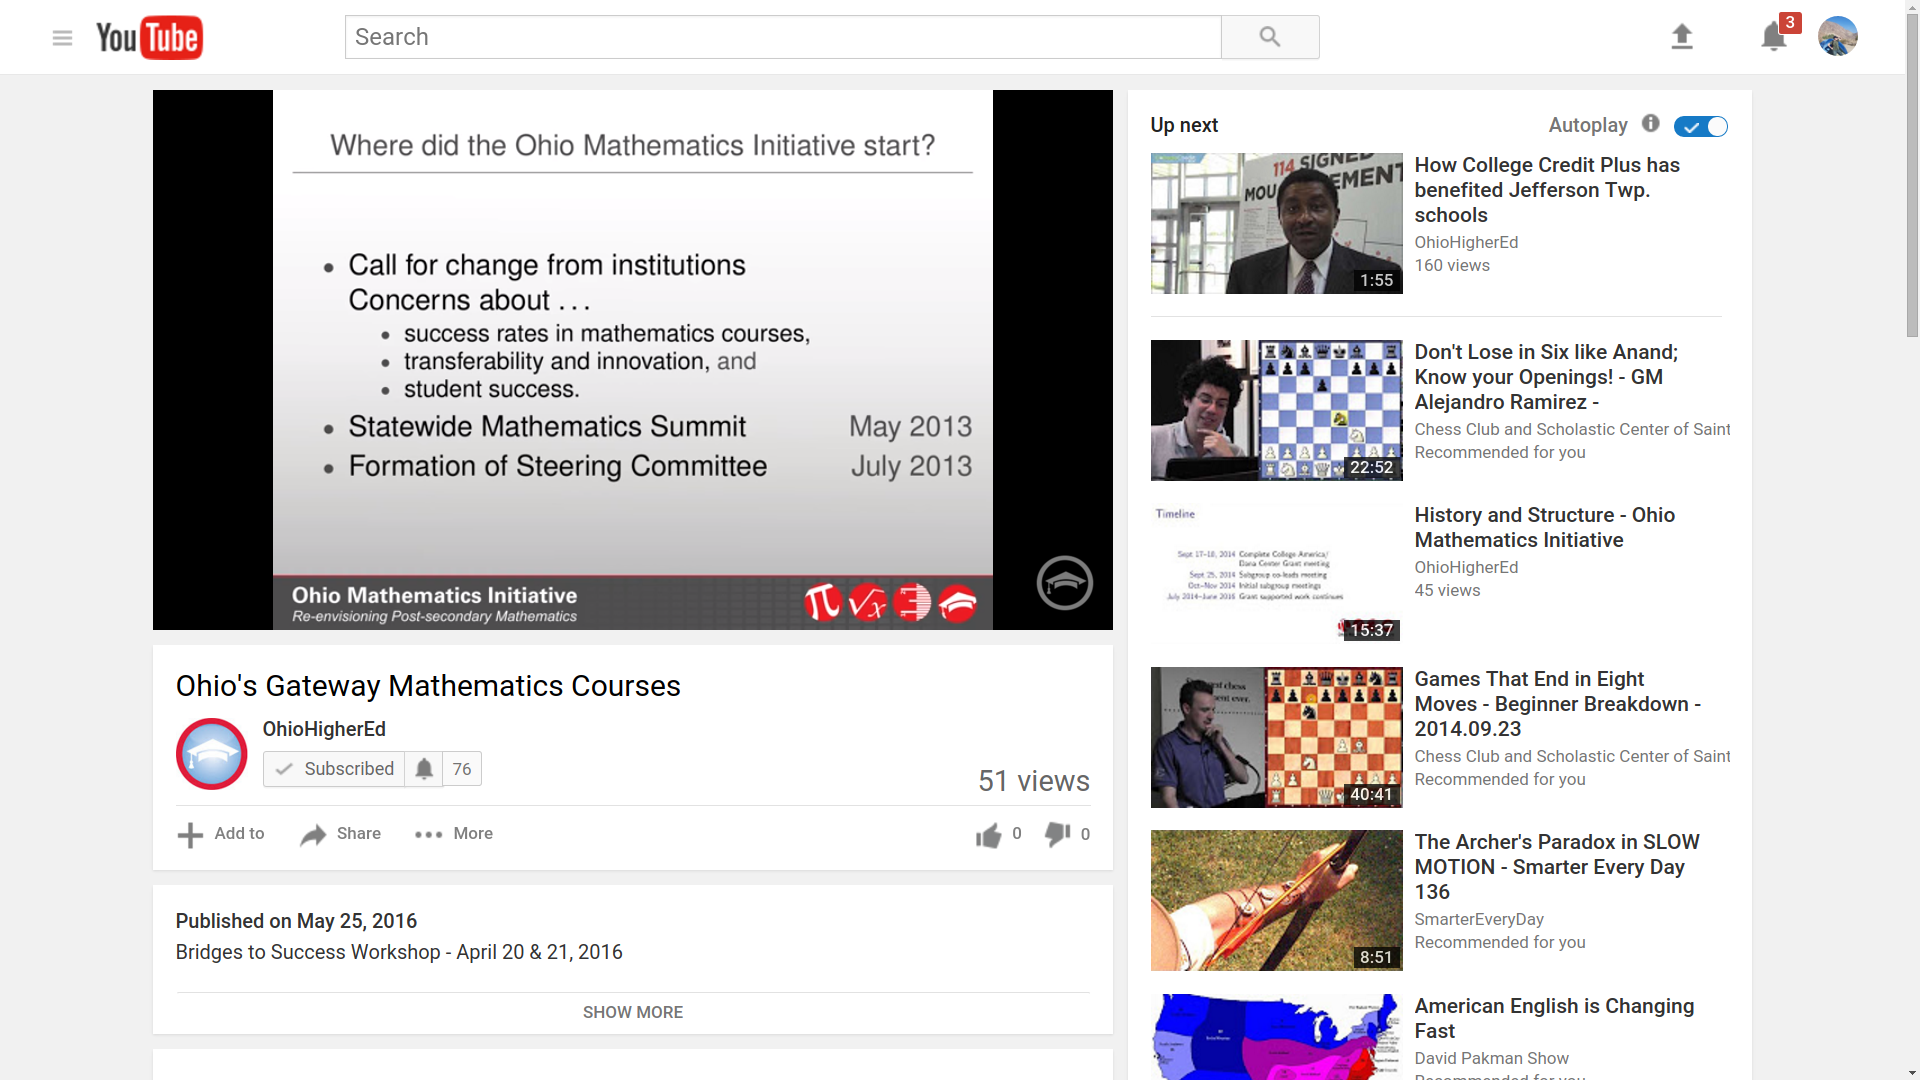
\includegraphics[width=0.7\textwidth]{video-screenshot.png}
\end{center}

\end{frame}


%%%%%%%%%%%%%%%%%%%%%%%%%%%%%%%%%%%%%%%%%%%%%%%%%%%%%%%%%%%%%%%%
\begin{frame}
\frametitle{Accomplishments since January 2016}

\textbf{Supporting OMI's publications}

The OMI published:
\begin{itemize}
  \item The FY16 Progress Report,
  \item The OMI---Overview 2016, \textcolor{gray}{and}
  \item The 2015--2017 Completion Initiatives Timeline.
\end{itemize}


\end{frame}

%%%%%%%%%%%%%%%%%%%%%%%%%%%%%%%%%%%%%%%%%%%%%%%%%%%%%%%%%%%%%%%%
\begin{frame}[allowframebreaks]

  \begin{center}
    \Huge Thank You!
  \end{center}

\end{frame}


\end{document}

